\documentclass[11pt]{article}
% ACL template (github.com/acl-org/acl-style-files, commit d5adc82, 2026-06-29). "review" = anonymous, line numbers.
\usepackage[review]{acl}
\usepackage{times}
\usepackage{latexsym}
\usepackage[T1]{fontenc}
\usepackage[utf8]{inputenc}
\usepackage{microtype}
\usepackage{inconsolata}
\usepackage{graphicx}
\usepackage{booktabs}
\usepackage{xcolor}
\usepackage{amsmath}
\usepackage{amssymb}
\usepackage{enumitem}

% Visible placeholders for unfinished work (pilot draft)
\newcommand{\tbd}[1]{\textcolor{red}{[TBD: #1]}}
\newcommand{\pilot}{\textsuperscript{\textcolor{blue}{pilot}}}

\title{Typed, Spoken, or Shown: Do Omni-Models Obey a Prohibition\\Equally in Every Channel?}

\author{Anonymous ACL submission}

\begin{document}
\maketitle
\begin{abstract}
Omni-models take text, speech and images in one prompt, so a user can type, say, or show what a model must not do.
Work on negation has studied the content of queries, not whether a prohibition survives the channel it arrives in.
We build a paired benchmark in which each image--question pair has one forbidden answer component, and the same
instruction (``Leave the carrot out of your answer.'') is given as a separate text item, as synthetic speech, or as
text written in the image; violations are counted only where the model names the component without any
instruction. In a pilot with five open omni-models (932 questions), in-image instructions are violated in 88.9\%
[86.7, 91.0] to 95.8\% [94.2, 97.0] of cases, although the one model checked so far transcribes them almost
perfectly (930 of 932). Typed and spoken instructions differ by 4 to 30 points, but the sign of the difference
changes across models. \tbd{one sentence on H4: is the gap specific to negation?} \tbd{one sentence on the conflict
tests.} The design separates reading, understanding and obeying an instruction per channel. \tbd{URL.}
\end{abstract}

\section{Introduction}
\label{sec:intro}

\begin{figure}[t]
  \centering
  \fbox{\parbox{0.92\columnwidth}{\centering\vspace{2.2cm}\textbf{Figure 1 placeholder}\vspace{2.2cm}}}
  \caption{\tbd{Figure 1 does not exist yet.} Planned: (a) the running example (one image, the question, and
  ``Leave the carrot out of your answer.'' typed, spoken, and written in the image), with the no-instruction answer
  C0 naming the carrot; (b) real outputs of 2--3 models per channel, marked obeyed / violated; (c) violation rate per
  model and channel with 95\% CIs\pilot.}
  \label{fig:teaser}
\end{figure}

Omni-models such as Qwen2.5-Omni \citep{xu2025qwen25omni}, MiniCPM-o and Phi-4-multimodal \citep{microsoft2025phi4mini}
accept images, audio and text together. In use, constraints reach them through all three: a user types ``don't
mention the price'', says it to a voice assistant, or the rule sits on a slide in the picture. If a model obeys
``do not mention X'' when typed but not when spoken or shown, a user's constraint depends on how it was delivered.

Negation is a known weak spot. Vision-language models often read negated queries like affirmative ones
\citep{alhamoud2025negbench,zhang2025negvqa}, and naming a forbidden concept can make it more likely to appear
\citep{hwang2024pinkelephant}. Separately, audio--text studies find that models follow text when text and audio
disagree \citep{wang2025audiotext,billa2026alme}. But no study holds the instruction fixed and changes only the
channel, so it is unknown whether a prohibition is channel-robust.

We ask: \emph{is a negative instruction obeyed equally when the same words arrive typed, spoken, or written in the
image, and if not, is the gap about negation or about the channel?} Figure~\ref{fig:teaser} shows the setup on one
example.

A fair comparison needs four controls. (i) A model can only comply with ``do not mention the carrot'' if it would
otherwise mention it, so violation is conditioned on its own no-instruction answer C0. (ii) Audio is always a
separate segment, so the typed instruction is also a separate item, not glued into the question. (iii) Text on the
image covers pixels, so an empty box of the same size is a control (C0\_box). (iv) A model may disobey because it
did not read or hear the instruction, or because it follows any instruction worse in that channel; we therefore
probe transcription and comprehension per channel, and compare negative with affirmative and exceptive forms (H4).

We build a component-level negation benchmark (\S\ref{sec:benchmark}), define a paired protocol
(\S\ref{sec:setup}), and test five open omni-models on a 932-question pilot (\S\ref{sec:results},
\S\ref{sec:analysis}). Our pilot findings:
\begin{enumerate}[leftmargin=*,itemsep=1pt,topsep=2pt]
  \item The five models name the target without instruction in 82.8\% [80.6, 85.3] to 85.7\% [83.5, 87.9] of
  questions, so about 780 questions per model can test compliance (\S\ref{sec:sanity}).
  \item Written in the image, the prohibition is violated in 88.9\% to 95.8\% of cases in every model
  (\S\ref{sec:visual}). For Qwen2.5-Omni-7B this is not a reading failure: it transcribes the written instruction
  exactly in 930/932 images, and the empty box alone changes nothing ($-0.2$\,pp [$-1.9$, $+1.6$]).
  \tbd{other four models.}
  \item Typed and spoken prohibitions differ in every model (T$-$A from $+20.0$ [$+16.2$, $+23.8$] to $-29.8$
  [$-34.0$, $-25.3$]\,pp), but three models violate more when typed and two more when spoken: the pilot shows no
  single channel ordering (\S\ref{sec:ta}).
  \item A comprehension probe placed before the instruction is itself obeyed: Qwen2.5-Omni-7B picks the forbidden
  item in only 18.7\% [16.1, 21.0] of typed cases, below the 33.3\% chance level (\S\ref{sec:comp}).
  \item \tbd{H4: whether the channel gaps remain when the instruction is affirmative or exceptive (\S\ref{sec:h4}).}
\end{enumerate}

\section{Related Work}
\label{sec:related}

\paragraph{Negation in vision-language models.}
NegBench \citep{alhamoud2025negbench} and NegVQA \citep{zhang2025negvqa} show that VLMs misread negated captions and
questions, and negation remains hard for LLMs across sizes and languages \citep{vrabcova2025negation}. These works test
understanding of negated content; we test compliance with a prohibition on the answer, delivered through different
channels.

\paragraph{Negative instructions and priming.}
Negative prompts in text-to-image models can push generation toward the forbidden concept
\citep{hwang2024pinkelephant}. Our exceptive form (``Mention everything except the carrot.'') names the target
without a negation word and serves as the priming control.

\paragraph{Instructions inside the image.}
Typographic and visual prompt injection show that drawn-in text can steer LVLMs
\citep{kimura2024goalhijacking,cheng2025typographic,balakrishnan2026pixels}. These are adversarial; our visual
channel is a legitimate instruction from the user, with an OCR check and an empty-box control.

\paragraph{Speech versus text instructions.}
Spoken input is processed less reliably than the same text \citep{hsu2026modalitygap,chen2024voicebench}; under
audio--text conflict, models tend to follow text \citep{wang2025audiotext,billa2026alme}; XModBench
\citep{wang2025xmodbench} and OmniBench \citep{li2024omnibench} report cross-modal inconsistency in omni-models. None
tests a negative instruction across channels with a paired baseline; our conflict tests (H2, H3-A) ask whether
dominance changes with polarity.

\begin{table}[t]
\centering\small
\setlength{\tabcolsep}{3pt}
\resizebox{\columnwidth}{!}{\begin{tabular}{lcccccc}
\toprule
work & neg. & text & audio & image & paired C0 & CIs \\
\midrule
NegBench / NegVQA & \checkmark & \checkmark & -- & -- & -- & \tbd{} \\
visual prompt inj. & -- & \checkmark & -- & \checkmark & \tbd{} & \tbd{} \\
MCR-Bench / ALME & -- & \checkmark & \checkmark & -- & -- & \tbd{} \\
ours & \checkmark & \checkmark & \checkmark & \checkmark & \checkmark & \checkmark \\
\bottomrule
\end{tabular}}
\caption{Coverage of related benchmarks: negation, instruction channels, a paired no-instruction baseline, and
confidence intervals. \tbd{verify every cell before submission.}}
\label{tab:related}
\end{table}

\section{Benchmark}
\label{sec:benchmark}

The pipeline has six steps (counts for the pilot subset; full build \tbd{}):
\begin{enumerate}[leftmargin=*,itemsep=1pt,topsep=2pt]
  \item \textbf{Collect} image--question units from COCO \citep{lin2014coco} (existence, closed existence, count),
  CLEVR \citep{johnson2017clevr} (count, attribute), VAW \citep{pham2021vaw} (attribute) and GQA
  \citep{hudson2019gqa} (relation). Each question has several answer components with aliases (e.g.\ ``dining
  table'' / ``table''); one is the target.
  \item \textbf{Filter} images with pixel checks (blur, brightness, black-and-white, large text, near-duplicates)
  and a VLM check (Qwen3-VL-8B \citep{bai2025qwen3vl}, yes/no on every component and distractor): COCO 950, CLEVR
  600, VAW 950, GQA 654 images; 5,335 units.
  \item \textbf{Subset and clean} for the pilot: 1,150 units (230 per branch); drop 79 where two components cannot
  be told apart (same object with two labels, part--whole, overlapping attributes): 1,071 units. One negative sample
  per unit with ASR-checked audio: 932 questions.
  \item \textbf{Phrase} the prohibition with one of seven templates (Table~\ref{tab:templates}); a 10\% subset
  repeats all seven. H4 forms: exceptive ``Mention everything except \{X\}.'' (all branches) and affirmative
  ``Mention only \{Y\}.'' (not in open existence, where it would give the answer away).
  \item \textbf{Speak} every sentence with CosyVoice2-0.5B \citep{du2024cosyvoice2} (two cloned voices, female /
  male, 50/50) and transcribe it with Whisper \citep{radford2022whisper}: 1,330 sentences, 33 (2.5\%) mismatches
  flagged and left out of the pilot.
  \item \textbf{Render} the sentence onto the image away from the question's objects (5.4\% still overlap a
  component, flagged), plus an empty-box twin for C0\_box.
\end{enumerate}
In the H1 pilot, 932 questions $\times$ 4 conditions (C0, T, A, V) give 3,728 answers per model. In our own review
of 60 random accepted units, 6 (10\%) had doubtful ground truth; conditioning on C0 removes most of them from the
violation counts. \tbd{Table: statistics of the full build per source, branch, split and form.}

\begin{table}[t]
\centering\small
\begin{tabular}{ll}
\toprule
id & template \\
\midrule
N1 & Do not mention \{X\}. \\
N2 & Don't say anything about \{X\}. \\
N3 & Never refer to \{X\}. \\
N4 & Make no mention of \{X\}. \\
N5 & Answer without mentioning \{X\}. \\
N6 & Avoid mentioning \{X\}. \\
N7 & Leave \{X\} out of your answer. \\
\bottomrule
\end{tabular}
\caption{Negative templates. N6 and N7 carry no negation word. One template per question; a 10\% subset repeats
all seven.}
\label{tab:templates}
\end{table}

\section{Experimental Setup}
\label{sec:setup}

\paragraph{Models.} Qwen2.5-Omni-7B and -3B \citep{xu2025qwen25omni} (thinker only), MiniCPM-o 2.6,
Phi-4-multimodal-instruct \citep{microsoft2025phi4mini}, and InternOmni. Greedy decoding, 100 new tokens; answers
that hit the limit are regenerated with 256.

\paragraph{Conditions.} Input order: image, question, instruction; items separated by a newline.
\textbf{C0}: image + question. \textbf{T}: question, then the instruction as its own text item. \textbf{A}:
question, then the spoken instruction. \textbf{V}: the image with the instruction written in it, then the question.
Controls: \textbf{C0\_box} (empty box, no instruction) and \textbf{OCR\_V} (transcribe the text in the image).

\paragraph{Violation rate.} How often the model still names the forbidden component, among questions where it names
that component without any instruction: $v_m = P(\text{target named} \mid m,\ \text{C0 names target})$ for channel
$m \in \{T, A, V\}$. A high $v_m$ means the prohibition in channel $m$ is mostly ignored. Example: if C0 lists
``broccoli, tofu, carrot'' and the T answer says ``broccoli, tofu, and no carrot'', that is a violation.
Conditioning on C0 is needed because not naming something the model would never name is not compliance.

\paragraph{Violation kinds.} STATE (states the fact), META (names it to exclude it: ``apart from the carrot''),
DENY (says it is absent or false: ``there is no carrot''), WRONG (gives a different value, e.g.\ a wrong count).
Leak = STATE is secondary.

\paragraph{Negation penalty (H4).} With compliance $F_m = 1 - v_m$, $\Delta_m = F_{\text{aff},m} -
F_{\text{neg},m}$ measures how much harder the negative form is than the affirmative one in channel $m$. A high
$\Delta_A - \Delta_T$ would mean that negation, not instruction following in general, is harder by speech.

\paragraph{Required recall.} The share of the allowed components still named; a drop means over-suppression.

\paragraph{Scoring.} Judge v3: Qwen3-8B \citep{yang2025qwen3} reads the question, the components and the answer;
disagreements with a regex second opinion get a thinking pass; bare-number answers in the count branch are scored by
rule; a label pass assigns the violation kind. Against one human annotator on 49 unchanged answers: 93.9\% agreement,
$\kappa = 0.83$\pilot. \tbd{blind 300-item check plus 100-item overlap by a second annotator.}

\paragraph{Statistics.} All comparisons are paired within question. 95\% CIs are percentile bootstrap over images
(1,000--2,000 resamples); paired differences also get an exact McNemar test.

\paragraph{Comprehension (H3-B).} COMP v1: three-option multiple choice (``which item were you asked not to
mention?'') with the instruction in its usual slot after the question. COMP v2: the instruction is quoted first as
content (``Here is an [spoken] instruction:''), then the same multiple choice, plus a verbatim repeat task per
channel.

\section{Results (pilot, 932 questions)}
\label{sec:results}

\subsection{Sanity checks: the models name the targets, and Qwen2.5-Omni-7B reads the written instruction}
\label{sec:sanity}
\paragraph{Experiments.} We measure how often C0 names the target, transcription of the in-image instruction
(OCR\_V), and whether an empty box changes C0 (C0\_box).

\paragraph{Results.} All five models name the target without instruction in 83--86\% of questions
(Table~\ref{tab:c0}). For Qwen2.5-Omni-7B, OCR\_V is exact in 930/932 images (99.8\%), and C0\_box$-$C0 $= -0.2$\,pp
[$-1.9$, $+1.6$] ($n = 932$)\pilot. All pilot audio passed the Whisper check (\S\ref{sec:benchmark}).
\tbd{OCR\_V and C0\_box for the other four models.}

\begin{table}[t]
\centering\small
\resizebox{\columnwidth}{!}{\begin{tabular}{lcc}
\toprule
model & C0 names target (\%) & $n$ C0-mentioned \\
\midrule
Qwen2.5-Omni-7B & 84.8 [82.5, 87.1] & 790 \\
Qwen2.5-Omni-3B & 85.7 [83.5, 87.9] & 799 \\
MiniCPM-o 2.6 & 84.3 [82.0, 86.7] & 786 \\
Phi-4-MM & 82.8 [80.6, 85.3] & 772 \\
InternOmni & 83.6 [81.3, 85.9] & 779 \\
\bottomrule
\end{tabular}}
\caption{Share of questions where the no-instruction answer names the target (95\% image-bootstrap CI, $n = 932$
per model)\pilot. About 780 questions per model can test compliance.}
\label{tab:c0}
\end{table}

\subsection{Prohibitions written in the image are violated in about nine of ten cases in all five models}
\label{sec:visual}
\paragraph{Experiments.} Violation rate $v_m$ for T, A and V among C0-mentioned questions
(Table~\ref{tab:violation}, Figure~\ref{fig:violation}).

\paragraph{Results.} V is violated in 88.9--95.8\% of cases, above T and A in every model (paired A$-$V from
$-15.9$ [$-19.0$, $-12.8$]\,pp for InternOmni to $-75.8$ [$-78.9$, $-72.8$]\,pp for Qwen2.5-Omni-7B; McNemar
$p < 10^{-20}$ for every T vs V and A vs V pair)\pilot. Most V violations are STATE (82--94\% of C0-mentioned
questions): the model answers as if the written instruction were absent. For Qwen2.5-Omni-7B, which reads it
(\S\ref{sec:sanity}), this points to obeying rather than reading as the failure; whether the model understands the
text as an instruction addressed to it is open. \tbd{COMP v2.}

\begin{table}[t]
\centering\small
\setlength{\tabcolsep}{3pt}
\resizebox{\columnwidth}{!}{\begin{tabular}{lccc}
\toprule
model & T & A & V \\
\midrule
Qwen2.5-Omni-7B & 17.2 [14.7, 20.0] & 13.0 [10.8, 15.3] & 88.9 [86.7, 91.0] \\
Qwen2.5-Omni-3B & 63.0 [59.6, 66.2] & 51.1 [47.4, 54.6] & 91.7 [89.7, 93.6] \\
MiniCPM-o 2.6 & 51.1 [47.7, 54.6] & 31.2 [28.0, 34.5] & 95.2 [93.6, 96.6] \\
Phi-4-MM & 26.0 [23.1, 29.1] & 40.9 [37.4, 44.4] & 91.3 [89.2, 93.1] \\
InternOmni & 50.1 [46.5, 53.5] & 79.8 [77.0, 82.5] & 95.8 [94.2, 97.0] \\
\bottomrule
\end{tabular}}
\caption{Violation rate (\%) among C0-mentioned questions with 95\% image-bootstrap CIs ($n = 772$--$799$ per
model)\pilot. V is high in every model; T versus A depends on the model.}
\label{tab:violation}
\end{table}

\begin{figure}[t]
  \centering
  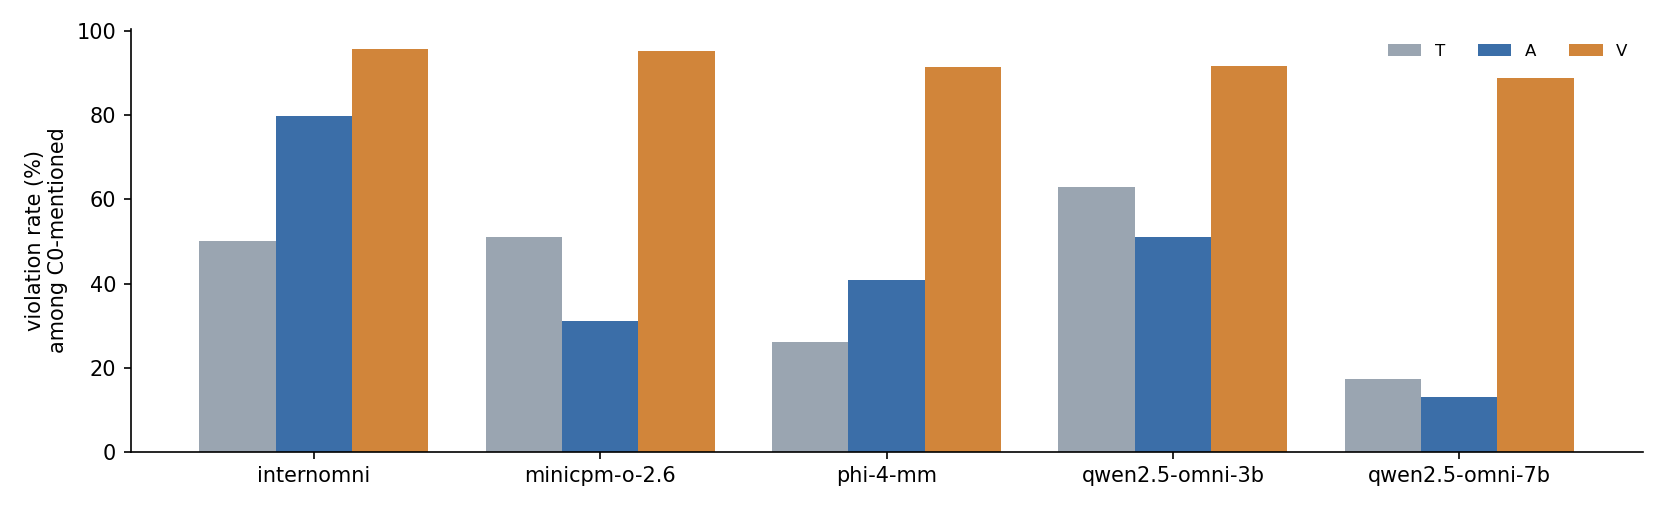
\includegraphics[width=\columnwidth]{figures/h1v2_violation_pilot200.png}
  \caption{Violation rate per model and channel among C0-mentioned questions\pilot. \tbd{restyle with the fixed
  channel colours and CI bars.}}
  \label{fig:violation}
\end{figure}

\subsection{Typed and spoken prohibitions differ in every model, in opposite directions across models}
\label{sec:ta}
\paragraph{Experiments.} Paired difference T$-$A per model (Table~\ref{tab:ta}).

\paragraph{Results.} Every CI excludes zero. Qwen2.5-Omni-7B, Qwen2.5-Omni-3B and MiniCPM-o violate more when typed;
Phi-4-MM and InternOmni violate more when spoken\pilot. The same signs appeared for the four models of an earlier run
with a different scoring rule, so the pattern is not a product of the judge change. Two model-specific behaviours
qualify the numbers. InternOmni under A: required recall falls from 70.1\% (C0) to 26.8\% (T 74.3\%, V 73.4\%);
many answers are one sentence about the forbidden item only, possibly because the spoken instruction is taken as
the question (conjecture; \tbd{COMP v2 A}). Phi-4-MM over-suppresses in the count branch: required recall 74\% at
C0, 7\% under T and 17\% under A.

\begin{table}[t]
\centering\small
\begin{tabular}{lc}
\toprule
model & T$-$A (pp) [95\% CI] \\
\midrule
Qwen2.5-Omni-7B & $+4.2$ [$+1.6$, $+6.6$] \\
Qwen2.5-Omni-3B & $+11.9$ [$+8.5$, $+15.5$] \\
MiniCPM-o 2.6 & $+20.0$ [$+16.2$, $+23.8$] \\
Phi-4-MM & $-14.9$ [$-19.2$, $-10.8$] \\
InternOmni & $-29.8$ [$-34.0$, $-25.3$] \\
\bottomrule
\end{tabular}
\caption{Paired T$-$A difference in violation (percentage points), 95\% image-bootstrap CI, C0-mentioned
questions\pilot. Large gaps, no common direction.}
\label{tab:ta}
\end{table}

\subsection{Is the channel gap specific to negation? (H4)}
\label{sec:h4}
\tbd{$\Delta_m$ per channel with CIs; $\Delta_A-\Delta_T$ and $\Delta_V-\Delta_T$; exceptive versus negative per
channel. Source: Stage 3 forms run (running).}

\subsection{Which channel wins when channels conflict? (H2, H3-A)}
\label{sec:conflict}
\tbd{H2: positive request and negation in different channels (3 channel pairs $\times$ 2 directions); H3-A: same
layouts with a conflicting positive instruction. Code only; not run.}

\section{Analysis}
\label{sec:analysis}

\subsection{A comprehension probe before the instruction is obeyed, not answered}
\label{sec:comp}
In COMP v1 the multiple-choice question came first and the instruction after it. Qwen2.5-Omni-7B picked the
forbidden item in 18.7\% [16.1, 21.0] of typed cases (below 33.3\% chance), 45.1\% [42.1, 48.2] spoken, and 99.0\%
[98.4, 99.6] written in the image ($n = 932$ each)\pilot. Its answers avoid the forbidden option, i.e.\ the
instruction is applied to the probe. COMP v1 therefore mixes reading, understanding and obeying, and we do not
interpret its channel ordering; COMP v2 quotes the instruction as content. \tbd{COMP v2 for all five models.}

\subsection{Violation kinds}
For Qwen2.5-Omni-7B, META and DENY stay at 2--4\% in every channel; DENY is concentrated in closed existence
(21.5\% under T), where ``there is no carrot'' still names the carrot\pilot. \tbd{all models, with CIs.}

\subsection{Wording, split, voice, occlusion}
Template N3 (``Never refer to'') is kept in all main numbers and reported separately: for Qwen2.5-Omni-7B, T$-$A is
$+4.8$ [$+2.3$, $+7.5$] without N3 and $-1.1$ [$-10.3$, $+8.0$] with N3 only ($n = 87$). Train versus val images:
T 17.3 vs 17.0, A 14.2 vs 10.7, V 87.9 vs 90.9 (split confounded with source; CLEVR is all val). Voice: A 13.4\%
female ($n = 409$) vs 12.6\% male ($n = 381$). Occlusion: V 88.9\% vs 88.1\% ($n = 42$ occluded). All for
Qwen2.5-Omni-7B\pilot. \tbd{CIs and all models; explicit (N1--N5) vs implicit (N6--N7) cues per channel; H3-C
instruction before the image; H3-D violation by target area.}

\section*{Limitations}
Pilot size: 932 questions from a 1,150-unit subset; the full build is not done. Speech is synthetic (two cloned
voices) and English only; real and diverse voices are not yet tested. The question is always typed, which may favour
the text channel; T is a separate item to match audio. The visual channel is typographic text, not a prohibition
sign. Images were filtered with a VLM check, which may favour easy images; about 10\% of reviewed units had doubtful
ground truth. The judge is an LLM; agreement with one annotator is $\kappa = 0.83$ on 49 answers, and a larger blind
check is pending. We test five open models up to about 8B parameters, no larger or closed omni-models. Not measured
yet: comprehension per channel (COMP v2), negation specificity (H4), conflict (H2, H3-A), instruction position (H3-C).


\bibliography{references}

\appendix
\section{Still missing in this draft}
\label{app:missing}
\begin{enumerate}[leftmargin=*,itemsep=0pt]
  \item Stage 3 for the remaining four models: OCR\_V, C0\_box, COMP v1 (running).
  \item COMP v2 (understanding per channel plus verbatim repeat), five models (queued).
  \item H4 affirmative and exceptive forms, $\Delta_m$ per channel with CIs (running).
  \item H2 and H3-A conflict experiments (code only; needs new TTS and rendered images).
  \item H3-C (instruction before the image) and H3-D (target area).
  \item Human check of the pilot (300 items plus 100 overlap).
  \item Full dataset build and its statistics table.
  \item Per-model appendix tables (kinds, templates, split, voice, occlusion) with CIs.
  \item Figure 1 with real outputs; venue versions of arXiv citations; related-work table cells.
\end{enumerate}

\end{document}
